\section{Deep Clustering}\label{sec:deep_clustering}

One of the holy grails of machine learning is achieving a general clustering algorithm, as retrieving labelled samples is often a very costly process. In some cases, labelled data is unavailable altogether. This is the case for some of the AT-TPC experiments, and so discovering clustering algorithms for event data is of some academic interest. 

Clustering algorithms based on neural networks are known collectively as deep clustering algorithms. Many of which are based on autoencoder architectures. In this thesis, we will focus on two such algorithms: the deep clustering with convolutional autoencoders (DCEC) algorithm, developed by \citet{Guo2017}. Also, the mixture of autoencoders (MIXAE) model, developed by \citet{Zhang}. 

\subsection{Deep Clustering With Convolutional Autoencoders}

The DCEC architecture is at its core a simple convolutional autoencoder. To convert it to a clustering algorithm, \citet{Guo2017} adds a fully connected transformation to a soft class assignment and a loss term for that assignment. 

To describe the DCEC we begin by letting the convolutional autoencoder be given in terms of the encoder $\psi(\boldsymbol{z}|\boldsymbol{x} ; \theta_e)$ and decoder $\phi(\boldsymbol{x}|\boldsymbol{z}; \theta_d)$, where the $\theta$ indicates the neural network parameters and $z \in \R^D$. Furthermore let the algorithm maintain $K$ cluster centers $\{\boldsymbol{\mu}_j\}^K$, where $j \in [0,\, 1,\, \dots,\, N]$ denote the clusters. These cluster centres are trainable parameters which map the latent samples to a soft assignment by a Student's t-distribution, in the model we parametrize them with a matrix $\mu_{ij}$. The assignment is then given as 

\begin{equation}\label{eq:qij}
q_{ij} = \frac{(1 + ||\boldsymbol{z}_i - \boldsymbol{\mu}_j||^2_2)^{-1}}{\sum_j(1 + ||\boldsymbol{z}_i - \boldsymbol{\mu}_j||^2_2)^{-1}}.
\end{equation}

\noindent The matrix elements $q_{ij}$ are then the probability of the latent sample $\boldsymbol{z}_i$ belonging to cluster $j$. A schematic of the model is shown in figure \ref{fig:dcec} to illustrate the structure of the DCEC model. 

To define the clustering loss over the soft assignments, we must first compute a target distribution $p_{ij}$. This distribution represents the confidence of the assignment $q_{ij}$. We define the 'target distribution as 

\begin{equation}
p_{ij} = \frac{q_{ij}^2/\sum_i q_{ij}}{\sum_j q_{ij}^2/\sum_i q_{ij}}.
\end{equation}

\noindent It is important to note that these distributions are not chosen arbitrarily. The soft assignments are computed in a way that is analogous to the t-SNE method described by \citet{VanDerMaaten2008}. Furthermore, the distribution $p_{ij}$ is chosen to improve cluster purity and emphasize the assignments with high confidence, according to \cite{Xie2016}. The loss is then computed as the KL-divergence between $p_{ij}$ and $q_{ij}$, i.e

\begin{equation}
\mathcal{L}_z = D(P ||Q ) = \sum_i \sum_j p_{ij} \log \frac{p_{ij}}{q_{ij}}.
\end{equation} 

\noindent \citet{Guo2017} show that the target distribution should not be updated with each epoch. Instead, it needs to be changed on a regular schedule. They found that for the handwritten digits dataset MNIST a suitable update was once every $T=140$ epochs. 

\begin{figure}[tb]
	\centering
	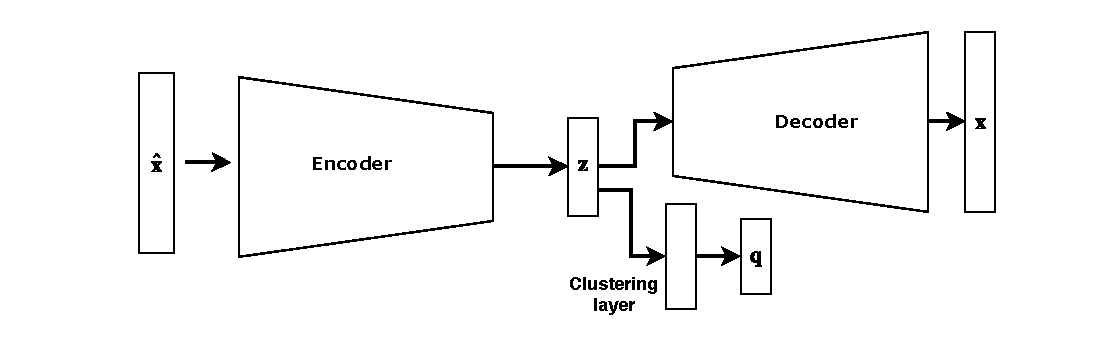
\includegraphics[width=\textwidth]{plots/dcec.pdf}
	\caption[Deep convolutional embedded clustering schematic]{Schematic of a DCEC model. A sample $\hat{\boldsymbol{x}}$ is compressed to a lower-dimensional representation $\boldsymbol{z}$. The latent sample is then fed both to a decoder which reconstructs the input, but also to a clustering layer which computes the soft assignments $\boldsymbol{q}$. See the text for further details. Figure adapted from \citet{Guo2017}}
	\label{fig:dcec}
\end{figure}

Training the DCEC algorithm is split into two phases. First, the convolutional autoencoder is trained until convergence with no regularization on the latent space. Secondly, the cluster centres are initialized using a k-means algorithm and which is then used to compute the target distribution for the first $T$ epochs. Lastly, the algorithm is trained with the KL-divergence loss and the original reconstruction term. We can then write the total cost as the sum of the reconstruction, $\mathcal{L}_x$, and clustering-loss, $\mathcal{L}_z$ as 

\begin{equation}
\mathcal{L} = \mathcal{L}_x + \gamma \mathcal{L}_z,
\end{equation}

\noindent where $\gamma$ is a weighting term for the clustering loss. \cite{Guo2017} empirically set $\gamma=0.1$ for their experiments. 

The fundamental challenge that DCEC faces is that it is dependent on a K-means solution that is good enough after the pre-training of the convolutional autoencoder. As the K-means algorithm is susceptible to outliers, scale differences in the latent axes,  and assumes that the clusters are isotropic Gaussians. 

\subsection{Mixture of autoencoders}\label{sec:mixae}

Another way of representing the clusters is by having multiple latent spaces representing the underlying manifolds that describe each class. This is the central idea in the Mixture of autoencoders (MIXAE) algorithm, introduced by  \cite{Zhang}. To ensure that each autoencoder represents a cluster, we attach a soft-max classifier to the set of latent samples. Recall from equation \ref{eq:softmax} that the soft-max function transforms a network output to a prediction of relative confidences. This classifier assigns a cluster to each autoencoder, coupling the latent space and the reconstructions. The soft-max classifier is trained to output cluster probabilities and penalized for collapsing to assigning one cluster only. The remaining task is then to connect the cluster assignments to the autoencoder reconstructions. This is achieved by multiplying by the cluster confidence with the reconstruction error of each autoencoder.

\begin{figure}[tb]
	\centering
	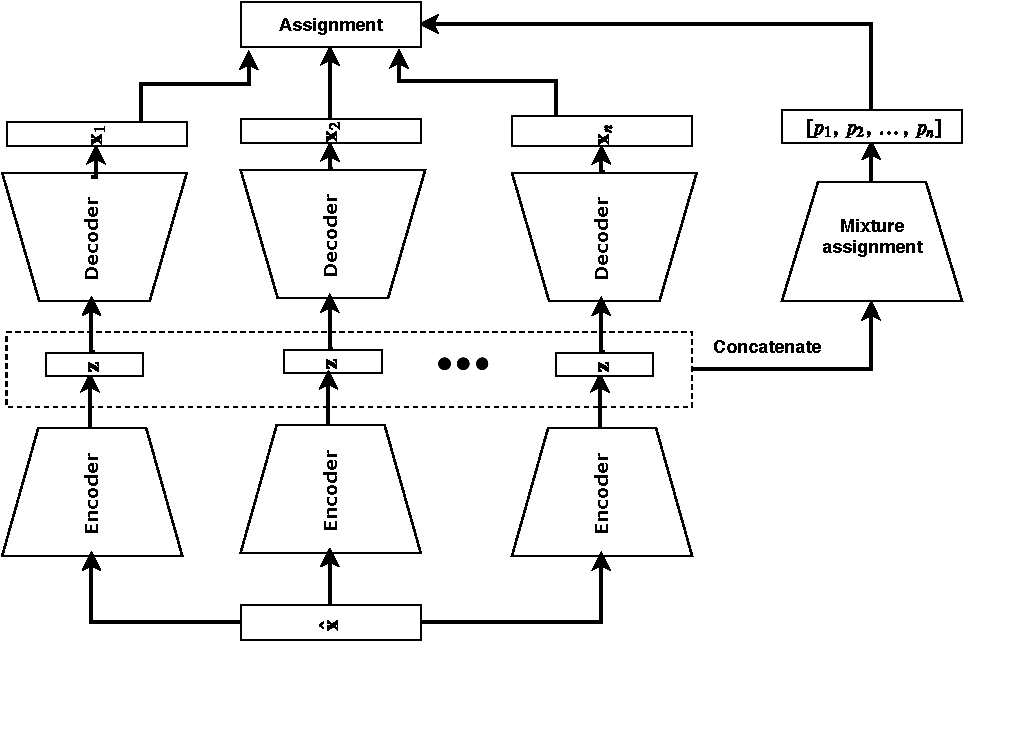
\includegraphics[width=\textwidth]{plots/mixae.pdf}
	\caption[Deep convolutional embedded clustering schematic]{Schematic of a DCEC model. A sample $\hat{\boldsymbol{x}}$ is compressed to set of lower-dimensional representations $\{\boldsymbol{z}^{(i)}\}$ by $N$ autoencoders. These samples are concatenated and passed through an auxiliary assignment network that predicts a confidence of cluster belonging for each autoencoder. For further details see the text. Figure adapted from \citet{Zhang}}
	\label{fig:mixae}
\end{figure}


More formally let $\{\boldsymbol{z}_j^{(i)}\}^N$ be the set of $N$ latent samples from each of the $N$ auto-encoders from a single sample image $\hat{\boldsymbol{x}}^{(i)} \in \R ^{t\times v}$ with height $t$ and width $v$. Furthermore, let the soft cluster assignments be given as $\{p_j^{(i)}\}^N$ and the reconstructed samples be given as $\{\boldsymbol{x}_j^{(i)}\}$. The reconstruction loss is then the sum over each autoencoder multiplied with each cluster assignment, i.e.

\begin{equation}\label{eq:mixae_reconst}
\mathcal{L}_x = \sum_j p_j^{(i)} \mathcal{C}(\boldsymbol{x}_j^{(i)}, \hat{\boldsymbol{x}}^{(i)}),
\end{equation}

\noindent where $\mathcal{C}(\cdot)$ is a cost function like the mean squared error or a cross-entropy.

We ensure that the soft cluster assignments encourage clustering by adding two terms to the total loss. The first is a simple entropy term which, when minimized, encourages the assignments to be one-hot vectors. Mathematically this loss can then be written as the entropy $S(\cdot)$ of a cluster assignment $\boldsymbol{p}$

\begin{equation}\label{eq:mixae_sample}
S(\boldsymbol{p}^{(i)})_{\text{sample}} = -\sum_j p_j^{(i)} \log p_j^{(i)}. 
\end{equation}

\noindent The last ingredient in the loss is then the term which discourages the trivial solution where only one cluster is being assigned. This loss is a batch-wise entropy term, given a mini-batch of $\beta$ samples the loss is computed as 

\begin{equation}\label{eq:mixae_batch}
\begin{split}
S(\{\boldsymbol{p}^{(i)}\}_i)_{\text{batch}}&= \left(-\sum_j \bar{p}_j \log \bar{p}_j \right)^{-1},\\
\bar{\boldsymbol{p}} &= \frac{1}{\beta} \sum_i ^\beta \boldsymbol{p}^{(i)} .
\end{split}
\end{equation}

\noindent The negative exponent in equation \ref{eq:mixae_batch} owes to the fact that we want to maximize the batch-wise entropy.

From equations \ref{eq:mixae_reconst}, \ref{eq:mixae_sample}, and \ref{eq:mixae_batch} we can then compose the full loss for the MIXAE model. \cite{Zhang} note that the optimization depends heavily on the weighting of the different terms and so we introduce the weighting hyperparameters $\alpha$, $\gamma$ and $\theta$, and write the total loss over a mini-batch as 

\begin{equation}\label{eq:mixae_loss}
\begin{split}
\mathcal{L}_{\text{total}}(\{\hat{\boldsymbol{x}}^{(i)}\}^\beta_i) = \frac{1}{\beta}\sum_i \Big( &\frac{t\cdot v}{\theta} \mathcal{L}_x(\boldsymbol{p}^{(i)},\,\boldsymbol{x}^{(i)},\, \hat{\boldsymbol{x}}^{(i)} ) \\
&+ \alpha S(\boldsymbol{p}^{(i)})_{\text{sample}} \Big) \\
&+\gamma S(\{\boldsymbol{p}^{(i)}\}_i)_{\text{batch}}.
\end{split}
\end{equation}

\noindent \citet{Zhang} note that this algorithm has a couple of shortcomings. The batch-entropy term encourages the cluster assignments to be uniformly distributed within the classes. However, it does have a second minimum when the assignments are all equally likely. For biased datasets with significant variations in the number of samples in each class, this can create problems for the algorithm. Additionally, the number of clusters are not dynamically computed by the algorithm but hard-coded by the researchers. This can be problematic if the number of cluster are not known prior to analysis.
